\chapter{Evaluation and Comparison of Automatic Metrics}
\label{metrics}

% \XXX{Pretavit abstrakt do nejakeho uvodu}
%
% Puvodni abstrakt, neco z toho dat do vlastniho abstraktu
%
% This paper presents the results of the WMT14 Metrics Shared Task. We asked
% participants of this task to score the outputs of the MT systems involved in
% WMT14 Shared Translation Task. We collected scores of 23 metrics from 12
% research groups. In addition to that we computed scores of 6 standard metrics
% (BLEU, NIST, WER, PER, TER and CDER) as baselines. The collected scores were
% evaluated in terms of system level correlation (how well each metric's scores
% correlate with WMT14 official manual ranking of systems) and in terms of
% sentence level correlation (how often a metric agrees with humans in comparing
% two translations of a particular sentence).

Automatic machine translation metrics play a very important role in the
development of MT systems and their evaluation. There are many different
metrics of diverse nature and one would like to assess their quality. For this
reason, the Metrics Shared Task is held annually at the Workshop of Statistical
Machine Translation\footnote{\url{http://www.statmt.org/wmt13}}, starting with
\perscite{koehn-monz:2006:WMT} and following up to
\perscite{wmt14-overview-paper}. In WMT13, we took over the organization of the
task \parcite{machacek:2013} and continued to do that also in WMT14
\parcite{machacek:2014}. In this chapter, we present the results of WMT14
metrics shared task with some additional information and comments.

In this task, we asked metric developers to score the outputs of WMT14 Shared
Translation Task \parcite{wmt14-overview-paper}. We have collected the computed
metrics' scores and use them to evaluate the quality of the metrics.  There are
actually two subtasks: a system-level task and a sentence-level task.

\begin{itemize}

    \item \textbf{System-level task.} In this subtask, participants compute one
      score for the whole test set, as translated by each of the systems. We
      then measure the correlation of those scores with the systems' official
      human scores.  The goal of metrics in this subtask is to give an overall
      ranking of the systems as close as possible to the official ranking
      according to human scores in each direction.
    
    \item \textbf{Sentence-level task.} In this subtask, participants compute
      one score for each sentence of each system's translation. We then measure
      the correlation of these scores with pairwise human judgements. The goal
      of metrics in this subtask is to compare two candidate sentences in the
      same way as humans would.

\end{itemize}

In the previous years, a lot of metrics performed very well in the system-level
task. In some of the translation directions, they predicted the overall ranking
of systems almost perfectly. However, there is still space for metrics to
improve.  In contrast to the system-level task, the sentence-level task is much
more difficult. The correlations in previous years were very low. It is
therefore very interesting to see whether metrics perform better this year.

The systems' outputs, human judgements and evaluated metrics are summarized in
Section \ref{section:data}. In Section \ref{section:metrics:description}, we
describe the participated metrics in more detail. The quality of the metrics in
terms of system-level correlation is reported in Section \ref{system-level}.
The sentence-level correlations with a detailed discussion and a slight change in
the calculation compared to the previous year is reported in Section
\ref{segment-level}.

\section{Data}
\label{section:data}

We used the translations of MT systems involved in WMT14 Shared Translation
Task together with reference translations as the test set for the Metrics Task.
This dataset consists of 110 systems' outputs and 10 reference translations in
10 translation directions (English from and into Czech, French, German, Hindi
and Russian). For most of
the translation directions each system's output and the reference translation
contain 3003 sentences. For more details please see the WMT14 overview
paper \parcite{wmt14-overview-paper}. 

\subsection{Manual MT Quality Judgements}

During the WMT14 Translation Task, a large scale manual annotation was
conducted to compare the systems. We used these collected human judgements for
the evaluation of the automatic metrics. 

The participants in the manual annotation were asked to evaluate the system outputs
by ranking translated sentences relative to each other. For each source sentence
that was included in the procedure, the annotator was shown the outputs of five
systems to which he or she was supposed to assign ranks. Ties were allowed.

These collected rank labels for each five-tuple of systems were then interpreted
as 10 pairwise comparisons of systems and  used to assign each system a score
that
reflects how high that system was usually ranked by the annotators. Please see
the WMT14 overview paper for details on how this score is computed. You
can also find inter- and intra-annotator agreement estimates there.


\subsection{Participants of the Metrics Shared Task}

\begin{table*}[t]
  \small
  \begin{center}
    \begin{tabular}{rl}
      \textbf{Metric} & \textbf{Participant} \\
      \hline
      \metric{AMBER} & National Research Council of Canada \parcite{improving:amber} \\
      \metric{APAC} & Hokkai-Gakuen University \parcite{wmt14-metric-apac} \\
      \metric{BEER} & ILLC -- University of Amsterdam \parcite{wmt14-metric-beer} \\
      \metric{BLEU-NRC} & National Research Council of Canada \parcite{wmt14-metric-bleunrc} \\
      \metric{DiscoTK-*} & Qatar Computing Research Institute \parcite{wmt14-metric-discotk} \\
      \metric{ELEXR} & University of Tehran \parcite{wmt14-metric-elexr} \\
      \metric{LAYERED} & IIT, Bombay \parcite{wmt14-metric-layered} \\
      \metric{Meteor} & Carnegie Mellon University \parcite{wmt14-metric-meteor} \\
      \metric{Parmesan} & Charles University in Prague \parcite{wmt14-metric-parmesan} \\
      \metric{RED-*} & Dublin City University \parcite{wmt14-metric-red} \\
      \metric{tBLEU} & Charles University in Prague \parcite{wmt14-metric-tbleu} \\
      \metric{UPC-IPA} & Technical University of Catalunya \parcite{wmt14-metric-upc} \\
      \metric{UPC-STOUT} & Technical University of Catalunya \parcite{wmt14-metric-upc} \\
      \metric{VERTa-EQ} & University of Barcelona \parcite{wmt14-metric-verta} \\
      \metric{VERTa-W} & University of Barcelona \parcite{wmt14-metric-verta} \\
    \end{tabular}
  \end{center}
  \caption{Participants of WMT14 Metrics Shared Task}
  \label{participants}
\end{table*}

Table \ref{participants} lists the participants of WMT14 Shared Metrics Task,
along with their metrics. We have collected 23 metrics from a total of
12 research groups.

In addition to that we have computed the following two groups of standard
metrics as baselines: 

\begin{itemize}

\item \textbf{Mteval.} The metrics \metric{BLEU} \parcite{Papineni02bleu:a} and
    \metric{NIST} \parcite{Doddington:2002:NIST} were computed using the script
    \texttt{mteval-v13a.pl}\footnote{\url{http://www.itl.nist.gov/iad/mig//tools/}}
    which is used in the OpenMT Evaluation Campaign and includes its own
    tokenization.  We run \texttt{mteval} with the flag
    \texttt{-{}-international-tokenization} since it performs slightly better
    \parcite{machacek:2013}.

\item \textbf{Moses Scorer.} The metrics \metric{TER} \parcite{Snover06astudy},
    \metric{WER}, \metric{PER} and \metric{CDER} \parcite{Leusch06cder:efficient}
    were computed using the Moses scorer which is used in the Moses model
    optimization. To tokenize the sentences we used the standard tokenizer
    script as available in the Moses toolkit.


\end{itemize}

We have normalized all metrics' scores such that better translations get higher scores. 

\section{Descriptions of the Metrics}
\label{section:metrics:description}

In this section, we present short descriptions of some interesting metrics which
participated in the shared task.  Please see the cited papers for more details
about the metrics. Note that the description of the \metric{BLEU} metric
has been already presented in Subsection \ref{enhancing:bleu}.

\subsection{AMBER}

Metric \metric{AMBER} is developed by \perscite{improving:amber}. The abbreviation 
stands for ``A Modified Bleu, Enhanced Ranking metric''. This metric is based
on \metric{BLEU} metric because, as the authors explain, \metric{BLEU}

\begin{itemize}
    \item is language independent,
    \item can be computed quickly (important for tuning),
    \item seems to be the best tuning metric.
\end{itemize}

\noindent They want to improve the correlation with human judgments while
preserving the advantages which make \metric{BLEU} so popular.
The basic formula for this metrics follows:

\begin{equation*}
    AMBER = score \cdot penalty
\end{equation*}

\noindent where $penalty$ is a weighted geometric average of 10 various penalty
measures and $score$ is given by:

\begin{equation*}
    score  = \theta_1 \cdot AvgP
           + \theta_2 \cdot Fmean 
           + \theta_3 \cdot AvgF 
\end{equation*}

\noindent where $AvgP$ is a geometric average of n-gram precisions (this is the
same as in \metric{BLEU}), $Fmean$ is the F-measure computed on the average
n-gram precision and average n-gram recall (averages are computed across $n \in
\{1, \ldots, N\}$) and $AvgF$ is an average (across $n \in \{1, \ldots, N\}$)
of F-measures computed on n-gram precision and n-gram recall for given $n$.

This is the basic computation but the authors propose many more enhancements,
for example they propose 8 different preprocessing (normalization and
tokenization) methods which are used to compute \metric{AMBER} metric on each
method separately and then return the average of scores computed after applying
all the methods. All free parameters of this metric were manually tuned on a
development set.

While we agree that the authors managed to preserve the key properties of
\metric{BLEU} mentioned above, we think that one of the most popular properties
of \metric{BLEU} is its implementation simplicity which is definitely not
preserved in \metric{AMBER}. 

\subsection{BEER}

This metric is proposed by \perscite{wmt14-metric-beer}. The abbreviation
stands for ``BEtter Evaluation as Ranking''. Their metric model can employ
various features which measure the similarity of candidate and reference
translations from various aspects.  Individual features are then combined using
a simple linear interpolation of feature functions:

\begin{equation*}
    score(h,r) = \sum_i w_i \cdot \phi_i(h,r) = \vect{w} \cdot \vect{\phi}(h,r)
\end{equation*}

They propose two groups of features. For adequacy features, they use precision,
recall and F1-score features for each of the following entities: function
words, content words, all words and character n-grams for $n \in \{1, \ldots,
6\}$. The total number of all adequacy features is 27.

The second group of features are ordering features. They represent orderings as
permutations. One of the ordering features is Kendall's $tau$ distance to
monotone permutation. Other 5 ordering features are based on permutation trees
introduced by \perscite{zhang2007factorization}.

They tune the feature weights to get the best correlation with human sentence-level
judgments. Let $h_{good}$ and $h_{bad}$ be two hypothesis translations of a source
sentence with reference translation $r$ and, let $h_{good}$ be ranked better than
$h_{bad}$ by human judgments.  Given that the metric's model is linear, one can
derive:

\begin{eqnarray*}
    score(h_{good},r) > score(h_{bad},r) & \Leftrightarrow & \vect{w} \cdot \vect{\phi}(h_{good},r) > \vect{w} \cdot \vect{\phi}(h_{bad},r) \\
                                         & \Leftrightarrow & \vect{w} \cdot \vect{\phi}(h_{good},r) - \vect{w} \cdot \vect{\phi}(h_{bad},r) > 0 \\
                                         & \Leftrightarrow & \vect{w} \cdot \left( \vect{\phi}(h_{good},r) - \vect{\phi}(h_{bad},r) \right) > 0
\end{eqnarray*}

Using the last equation, a binary classification problem can be formulated.  For
each human pairwise comparison we have one positive training instance with the
feature vector $\vect{\phi}(h_{good},r) - \vect{\phi}(h_{bad},r)$ and one
negative training instance with the feature vector $\vect{\phi}(h_{bad},r) -
\vect{\phi}(h_{good},r)$. A regression is then used to train the
weight vector $\vect{w}$.

Please note that once the weight vector is trained, there is no need to
classify a pair of hypothesis when evaluating. A score of a single evaluated hypothesis $h$
is computed as $\vect{w} \cdot \vect{\phi}(h,r)$.



\subsection{BLEU-NRC}

The original \metric{BLEU} is not very suitable for evaluating single sentences. It
can easily happen that for higher values of $n$, no n-gram from the candidate
matches the reference translation. The precision is then zero and since
the \metric{BLEU} score is computed as the geometric average, it is also zero.
A lot of sentences therefore get zero scores and even they can be meaningful. There
is also a problem with very short sentences for which the precisions of higher
$n$ values could be undefined. To compute \metric{BLEU} on sentence level, one
has to smooth the precision values.

Let $m_n$ be the clipped count of n-grams occurring in both the reference and
candidate translations, and let $l_n$ be the total count of n-grams in the
candidate. In the original \metric{BLEU}, the precision is computed as $p_n = m_n /
l_n$. When smoothing, a modified clipped count $m_n'$ is computed and then the
precision is computed as $p_n = m_n' / l_n$. 

\perscite{wmt14-metric-bleunrc} compare various smoothing methods and choose
the method which correlates best with sentence-level judgments. Their best
performing smoothing method is a combination of two methods. They compute first
modified counts $m_n'$ and based on them, they compute second modified counts
$m_n''$.

The first modified counts are computed using the following algorithm:
\begin{algorithmic}[1] \Let{$invcnt$}{$1$} \For{$n$ \textbf{in} 1 \textbf{in}
    $N$} \If{$m_n = 0$} \Let{$invcnt$}{$invcnt \cdot \frac{K}{\ln(\len(c))}$}
    \Let{$m_n'$}{$1 / invcnt$} \Else \Let{$m_n'$}{$m_n$} \EndIf \EndFor
\end{algorithmic} where $K$ is set empirically (they use $K = 5$). The
assignment in line 4 means that for shorter sentences, the smoothed clipped
counts are smaller. The motivation for this is the fact that the denominator in
the precision computation is smaller for shorter sentences and therefore the
numerator should be also smaller so that precisions for shorter sentences are
not inflated. However, we think that this allows to game the metric by
producing very long sentences with no n-gram matched: if $\len{c} > e^K$, than
the variable $invcnt$ will decrease and the clipped counts $m_n'$ will
therefore increase. For each positive real number, there exists a sentence
length which would ensure the metric score to be higher than the given number.
We, however, do not consider this as a serious problem.

The second smoothing technique is used on top of the first method, and is inspired by
the intuition that matched counts for similar values of $n$ should be similar.
This method therefore computes the modified matched counts as an average of
neighbouring clipped counts. The authors define $m_0'' = m_1' + 1$ and
calculate $m_n''$ for $n > 0$ as follows:

\begin{equation*}
    m_n'' = \frac{
        m''_{n-1} + m_n' + m_{n+1}'
    }{
        3
    }
\end{equation*}

Finally, the n-gram precisions and the BLEU score are computed from the modified
clipped counts $m_n''$.

For completeness we also report how the \metric{BLEU} metric is smoothed in
the Moses MERT implementations since it is used for computing a baseline metric
\metric{sentBLEU} in the sentence-level results. To both the numerator and denominator
in the precision computation, a one is added:
\begin{equation*}
    p_n = \frac{
        m_n + 1
    }{
        l_n + 1
    }
\end{equation*}

\subsection{WER}

Word Error Rate metric is based on an edit distance. It is similar to the Levenshtein
distance but the edit operations work with tokens instead of characters and the edit
distance is normalized by the length of the reference $r$:

\begin{equation*}
    WER(c,r) = \frac{
        \min_{e \in E(c,r)} \left( D(e) + S(e) + I(e) \right)
    }{
        |r|
    }
\end{equation*}

\noindent where $E(c,r)$ denotes a set of all sequences of edit operations
which transform the candidate $c$ to the reference $r$, and $D(e)$, $S(e)$,
$I(e)$ denote the number of deletions, substitutions and insertions of tokens
respectively in the sequence $s$.

The minimal sequence can be easily computed using a dynamic programing algorithm.
This computation can be visualized with an alignment grid which you can see
in Figure \ref{wer-grid}.

\begin{figure}
    \begin{center}
        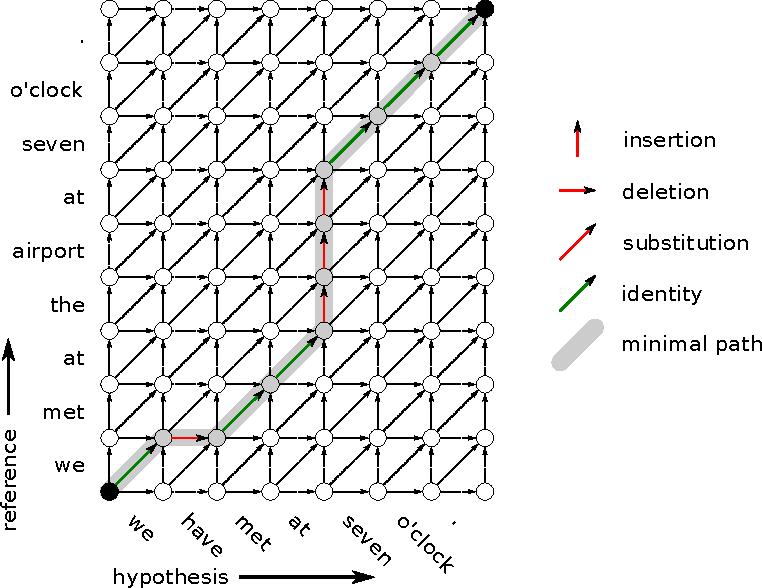
\includegraphics[width=10cm]{img/wer-grid.pdf}
    \end{center}

    \caption{An example of WER alignment grid}
    \label{wer-grid}
\end{figure}

\subsection{CDER}

The abbreviation of this metric stands for ``Cover Disjoint Error Rate'' and it
was developed by \perscite{Leusch06cder:efficient}. This metric is similar to
\metric{WER} in that it is also an edit distance based metric. In addition to the
insertions, substitutions and deletions, \metric{CDER} also allows long jumps.
The long jump is an operation in which we move in an alignment grid to any
position in the candidate (we can get to any position in the current row of the
alignment grid for a unit price). This simulates movements of blocks (longer
sequences of tokens) and it is motivated by that block movements should not be
penalized so harsh. The \metric{CDER} is computed as follows:

\begin{equation*}
    CDER(c,r) = \frac{
        \min_{e \in E(c,r)} \left( D(e) + S(e) + I(e) + LJ(e) \right)
    }{
        |r|
    }
\end{equation*}

\noindent where $E(c,r)$ denotes a set of all sequences of edit operations
which transform the candidate $c$ to the reference $r$, and $D(e)$, $S(e)$,
$I(e)$, $LJ(e)$ denote the number of deletions, substitutions, insertions and long
jumps respectively in the sequence $s$. You can see an example of an alignment grid with
long jumps in Figure \ref{cder-grid}.

\begin{figure}
    \begin{center}
        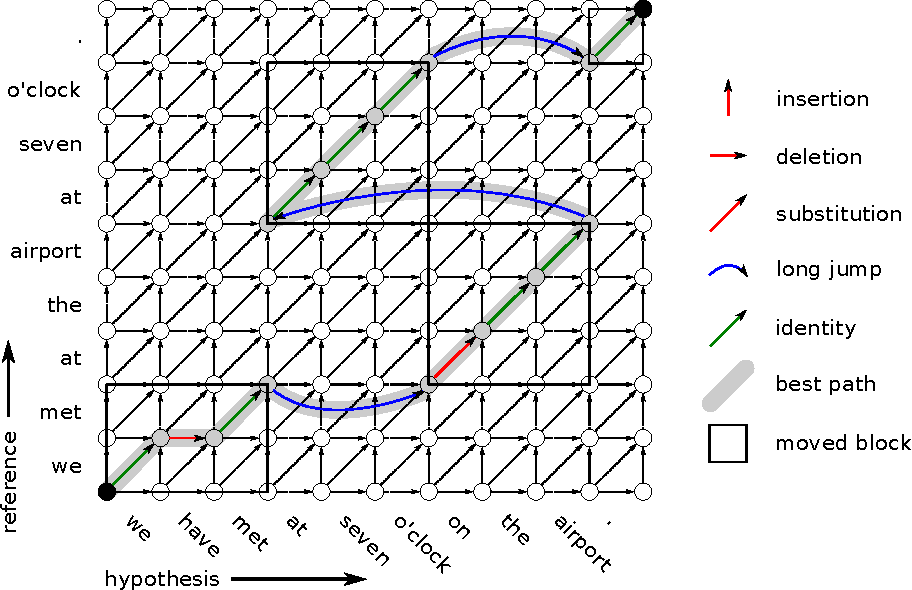
\includegraphics[width=12cm]{img/cder-grid.pdf}
    \end{center}

    \caption{An example of CDER alignment grid with long jumps}
    \label{cder-grid}
\end{figure}

\subsection{DiscoTK}

\metric{DiscoTK} metric family was developed by \perscite{wmt14-metric-discotk}.
Its abbreviation stands for ``Discourse Tree Kernel''. The basic principle is
that both reference and candidate translations are parsed to discourse parse
trees which are then compared using convolution tree kernels. There are 5
different discourse tree representations; all of them are compared and
normalized kernels scores are then averaged with uniform weights to get the
\metric{DiscoTK-light} score.  Please see the paper for more details.

One of the weaknesses of the above discourse-based metrics is that they use
unigram lexical information, which does not capture reordering. To make a more
robust metric, \perscite{wmt14-metric-discotk} combined the above five measures
with twelve more metrics implemented by \perscite{gimenez2010linguistic} in the
\textsc{Asiya} toolkit.\footnote{\url{http://nlp.lsi.upc.edu/asiya/}}. The 17
measures in total are then averaged with uniform weights to get
\metric{DiscoTK-party} score. The second variant of this metric,
\metric{DiscoTK-party-tuned}, averages the measures with tuned weights.

\subsection{LAYERED}

\metric{LAYERED} was developed by \perscite{wmt14-metric-layered}. Its name
comes from combining metrics on various linguistic layers:

\begin{itemize}

    \item \textbf{Lexical Layer.} The authors decided to use ordinary
        \metric{BLEU} from this layer.

    \item \textbf{Syntactic Layer.} \metric{LAYERED} employs three metrics
        working on this layer, 
        all of them are permutation based
        metrics and therefore consider only reordering of words. Permutations
        are constructed from source-candidate and source-reference alignments.
        The first two metrics are designed by \perscite{birch2011reordering}.

        The first metric is Hamming Score (HAMMING), which is a normalized
        Hamming distance defined as the number of disagreements between two
        permutations: $\left| \left\{ i \in \{1 \ldots n\} \mid \pi(i) \ne
        \sigma(i) \right\} \right|$. 

        The second metric is Kendall's $\tau$ distance (\metric{KTD}), which
        measures the minimum number of transpositions of two adjacent symbols
        necessary to transform one permutation into another.
        
        The last metric
        is Spearman rank correlation coefficient (\metric{SPEARMAN}), which
        measures how much the permutation between the candidate and the
        reference is monotone. (We also use Spearman rank correlation coefficient
        for the metrics evaluation. You can find the exact definition later in
        this chapter).

    \item \textbf{Semantic Layer.} There are two metrics working on this layer.
        Both of them compute precision and recall of matched dependencies in
        candidate and reference parse trees and then average them to get a
        single score.\footnote{A question is why the authors do not use
            F-measure which is usually used to combine precision and recall.
        They do not even use the terms precision and recall and instead
    define the concepts of precision and recall using a textual entailment
concept.}  The first metric (\metric{SHALLOW}) uses the Stanford dependency
parser \parcite{Marneffe06generatingtyped} to generate the dependencies. The
second metric (\metric{DEEP}) uses the UNL dependency graph generator to
construct the dependencies.

\end{itemize}

All the metrics from all the layers are then linearly combined (using tuned weights)
to get a final \metric{LAYERED} score: 

\begin{eqnarray*}
    LAYERED & = & 0.26 \cdot BLEU + 0.13 \cdot HAMMING + 0.03 \cdot KTD \\ 
            & + & 0.04 \cdot SPEARMAN + 0.28 \cdot SHALLOW + 0.26 \cdot DEEP 
\end{eqnarray*}

\subsection{Meteor}

\metric{Meteor} \parcite{wmt14-metric-meteor} evaluates candidate translations
in two phases. In the first phase, it aligns a candidate translation to a
reference translation. In the second phase, a sentence-level similarity score
is computed using the constructed alignment. 

When aligning the candidate and the reference translations, the words
(sometimes phrases) in the candidate are matched to the words (phrases) in the
reference using the following matchers:

\begin{itemize}
    \item \textbf{Exact:} Matches words if their surface forms are identical.
    \item \textbf{Stem:} Matches words if their stem is identical. A language appropriate
        stemmer is used.
    \item \textbf{Synonym:} Matches words if both of them are in any synonym set according 
        to the WordNet database.
    \item \textbf{Paraphrase:} Matches phrases if they are listed in a language appropriate 
        paraphrase table. These tables can be automatically extracted from ordinary phrase tables
        used in statistical machine translation. 
\end{itemize}

Since there could be more possible alignments, the final alignment is then
resolved as the largest subset of all matches which meets the following
criteria:

\begin{enumerate}
    \item Each word in each sentence has to be covered by zero or one match.
    \item The total number of matched words in each sentence is maximal.
    \item The number of chunks is minimal (chunk is a contiguous sequence of
        candidate words which is monotonically mapped to a contiguous
        sequence of reference words).
    \item An alignment with a smaller total sum of absolute distances between
        the positions of aligned words is preferred. 
\end{enumerate}

The \metric{METEOR} for an aligned sentence is then computed as follows. Let
$h_c$ and $h_f$ be content words and function words respectively in the
hypothesis (candidate translation), and similarly let $r_c$ and $r_f$ be
content and function words in the reference. For each of the matchers $m_i$
defined above, let $m_i(h_c)$, $m_i(h_f)$ be the counts of matched content and
function words in the hypothesis and similarly let $m_i(r_c)$, $m_i(r_f)$ be
the counts of matched content and function words in the reference. Finally
a weighted precision and recall are computed:

\begin{equation*}
    P = \frac{
        \sum_i w_i \cdot ( \delta \cdot m_i(h_c) + (1-\delta) \cdot m_i(h_c))
    }{
        \delta \cdot |h_c| + (1-\delta) \cdot |h_f|
    }
\end{equation*}

\begin{equation*}
    R = \frac{
        \sum_i w_i \cdot ( \delta \cdot m_i(r_c) + (1-\delta) \cdot m_i(r_c))
    }{
        \delta \cdot |r_c| + (1-\delta) \cdot |r_f|
    }
\end{equation*}

\noindent where $w_1 \ldots w_n$ are weights of the matchers and $\delta$ is a weight
controlling the importance of content words over function words.
Using the computed precision and recall, a F mean is computed:
\begin{equation*}
    F_{mean} = \frac{
        P \cdot R
    }{
        \alpha \cdot P + (1 - \alpha) \cdot R
    }
\end{equation*}

\noindent Finally, the \metric{Meteor} score is computed as follows:

\begin{equation*}
    METEOR = (1-Pen)\cdot F_{mean}
\end{equation*}

\noindent where $Pen$ is a fragmentation penalty calculated as 

\begin{equation*}
    Pen = \gamma \cdot \left( \frac{ch}{m} \right)^\beta
\end{equation*}

\noindent where $ch$ is the number of chunks (as defined above) and $m$ is the
total number of matched words. All the parameters $\alpha$, $\beta$, $\gamma$,
$\delta$ and $w_1 \ldots w_n$ are tuned to maximize the correlation with human
judgments.

Some of the \metric{Meteor} components need language specific resources.
While some of the resources are limited to one or a few languages, other
resources can be easily trained from bilingual or monolingual data. For
example, the list of function words consists of all words with relative
frequency above a certain treshold. Paraphrase tables are constructed with a
simple method from a phrase table. The weights are tuned for each language
direction independently, however developers of \metric{Meteor} have also tuned
a universal set of weights which can be used for any language direction. This
is the case, for example, for directions from Russian and Hindi. The results
for these directions are also very poor.

%\subsection{NIST}
%\subsection{Parmesan}
%\subsection{PER}
%\subsection{RED}
%\subsection{tBLEU}
\subsection{UPC}
\subsection{VERTa}

\section{System-Level Metric Analysis}
\label{system-level}

When evaluating metrics on the system level, we would like to reward metrics
which predict the ordering of the systems as similar as possible to the
ordering given by the human scores.

While the Spearman's $\rho$ correlation coefficient was used traditionally as
the main measure of system-level metrics' quality in the past, we have decided
to use Pearson correlation coefficient as the main measure this year. We give
reasons for this change in the next subsection.

Pearson correlation coefficient is a metaevaluation metric which measures how
much two variables are linearly correlated.  In our case, the first variable is
the human score and the second variable is the metric score. We use the
following formula to compute the Pearson's $r$ for each metric and translation
direction:

\begin{equation}
    r = \frac{\sum ^n _{i=1}(H_i - \bar{H})(M_i - \bar{M})}{\sqrt{\sum ^n _{i=1}(H_i - \bar{H})^2} \sqrt{\sum ^n _{i=1}(M_i - \bar{M})^2}} 
\end{equation}

\noindent where $H$ is the vector of human scores of all the systems translating in
the given direction and $M$ is the vector of the corresponding scores as predicted
by the given metric. $\bar{H}$ and $\bar{M}$ are their means respectively.

The Pearson's $r$ ranges from -1 to 1. A value of 1 implies that a linear
equation describes the relationship between the human scores and the metric
scores and the metric score increases as the human score increases. A value of
-1 also implies a linear relationship but this time the metric score decreases
as the human score decreases. A value of 0 implies that there is no
relationship between the human scores and the metric scores.

Since we have normalized all metrics such that better translations get a higher
score, we consider metrics with values of Pearson's $r$ closer to 1 as better. 

For the sake of completeness and for the possibility to compare the results to
previous years, we also report Spearman's rank correlation coefficient in the
tables. This metaevaluation metric measures how much the human score and the
metric score are mononotonically related.  This measure does not consider the
absolute differences between the values so the relationship between the two
variables is not penalized for not being linear.  To compute Spearman's $\rho$,
we must first transform the variables to ranks.  If there are some equal
values, we assign to them an average of corresponding ranks. Once we have the
ranks, we can compute Spearman's $\rho$ as the Pearson correlation coefficient
between the rankings. Since there are no tied scores, we use the following
simplified formula: \begin{equation*} \rho = 1 - \frac{6 \sum{d_i^2}}{n(n^2
-1)} \end{equation*} where $d_i$ is the difference between the human rank and
metric's rank for system $i$ and $n$ is number of the systems. The possible
values of $\rho$ range between 1 and -1. A value of 1 implies that the metric
scores give the same ranking of the systems as the official human scores. A
value of -1 implies that the metric scores give a reversed ranking.

The reported empirical confidence intervals of system-level correlations were
obtained through bootstrap resampling of 1000 samples (confidence level of
95\,\%).

\subsection{Reasons for Pearson correlation coefficient}

In the translation task, there are often similar systems with human scores very
close to each other. It can therefore easily happen that even a good metric
compares two similar systems differently from humans. We believe that the
penalty incurred by the metric for such a swap should somehow reflect that the
systems were hard to separate.

Since the Spearman's $\rho$ converts both human and metric scores to ranks and
therefore disregards the absolute differences in the scores, it does exactly what
we feel is not fair. The Pearson correlation coefficient does not suffer from this 
problem. We are aware of the fact that Pearson correlation coefficient also
reflects whether the relation between manual and automatic scores is linear (as
opposed to e.g. quadratic). We don't think this would be negatively affecting
any of the metrics since overall, the systems are of a comparable quality and
the metrics are likely to behave linearly in this small
range of scores.

\begin{figure}
    \begin{center}
        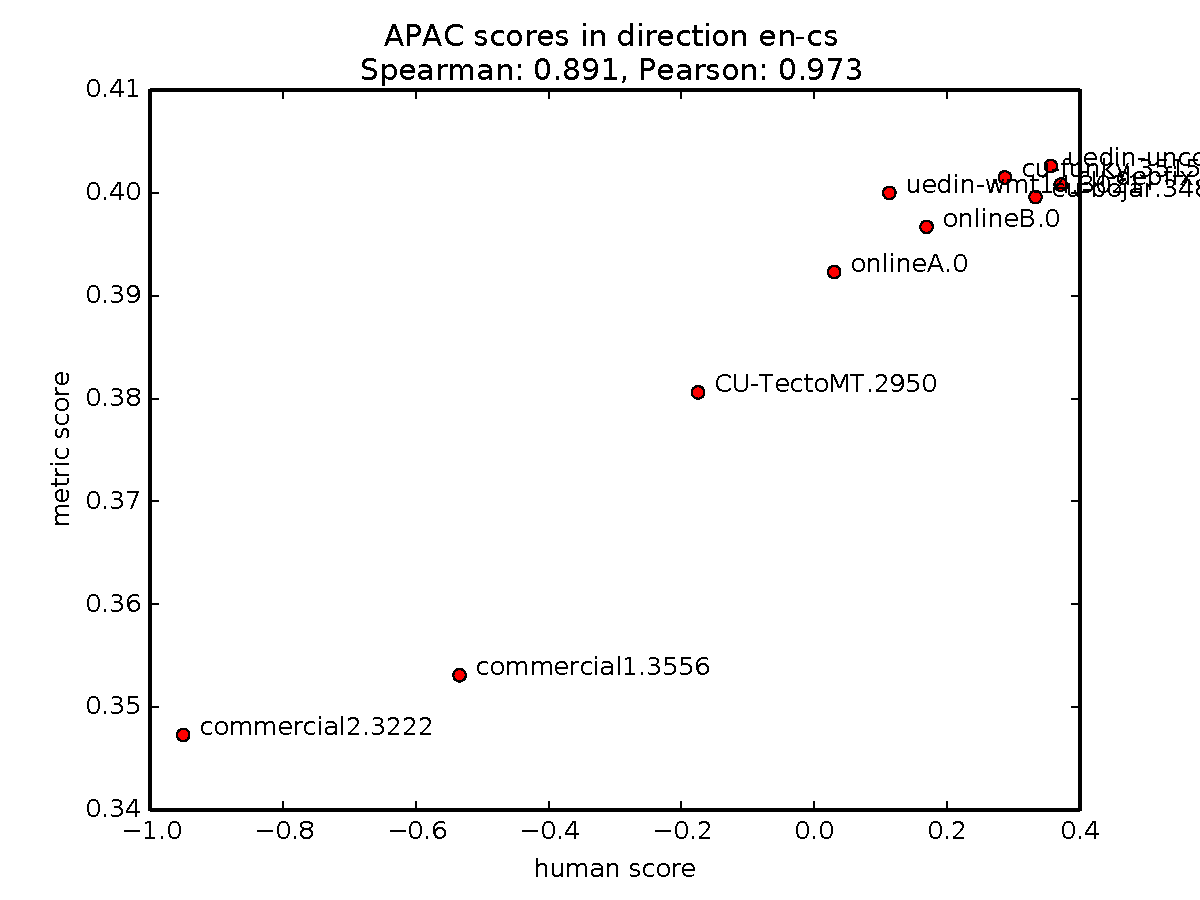
\includegraphics[width=\textwidth]{img/pearson-motivation.pdf}
    \end{center}

    \caption[Motivation for Pearson: Metric vs. human scores scatterplot]{
      Motivation for Pearson: Metric vs. human scores scatterplot
}

    \label{tree-align}
\end{figure}

You can see an example situation in Figure \ref{tree-align}. There is a cluster
of very similar systems in upper right corner. In this cluster, some systems
are not ranked correctly by the metric. For instance, the swap of the uedin-wmt14
and onlineB systems is not penalized so harsh in the Pearson score. However
in Spearman score, it is penalized just the same as a swap of very distant
systems would be penalized, for instance commercial1 and CU-TectoMT.


Moreover, the general agreement to adopt Pearson instead of Spearman's
correlation coefficient was already apparent during the WMT12 workshop. This
change just did not get through for WMT13.

\subsection{Results}

You can find the system-level correlations for translations into English in
Table \ref{system-level-corrs-toEn} and for translations out of English in
Table \ref{system-level-corrs-outEn}. Each row in the tables contains
correlations of a metric in each of the examined translation directions. The
metrics are sorted by average Pearson correlation coefficient across the
translation directions. The best results in each direction are in bold.

As in previous years, a lot of metrics outperformed \metric{BLEU} in system
level correlation. In into-English directions, the metric
\metric{DiscoTK-party-tuned} has the highest correlation in two language
directions and it is also the best correlated metric on average according to both
Pearson and Spearman's coefficients. The second best correlated metric on
average (according to Pearson) is \metric{LAYERED} which is also the single
best metric in Hindi-to-English direction.  Metrics \metric{REDSys} and
\metric{REDSysSent} are quite unstable, they win in French-to-English and
Czech-to-English directions respectively but they perform very poorly in other
directions. 

Except \metric{Meteor}, none of the participants took part in the last year's
metrics task.  We can therefore compare current and last year's results only for
\metric{Meteor} and baseline metrics.  \metric{Meteor}, the winner last year,
performs generally well in some directions but it suffers horribly when
evaluating translations from non-Latin script (Russian and especially Hindi).
For the baseline metrics the results are quite similar across the years. In
both years \metric{BLEU} performs best among baseline metrics, closely followed
by \metric{CDER}. \metric{NIST} is in the middle of the list in both
years. The remaining baseline metrics \metric{TER}, \metric{WER}
and \metric{PER} perform significantly worse.

The results into German are markedly lower and have broader confidence
intervals than the results in other directions. This could be explained by a
very
high number (18) of participating systems of similar quality. 
Both human judgements and automatic metrics are negatively affected by these
circumstances. To preserve the reliability of overall metrics' performance
across languages, we
decided to exclude English-to-German
direction from the average Pearson and Spearman's correlation coefficients.

In other out-of-English directions, the best correlated metric on average according
to Pearson coefficient is \metric{NIST}, even though it does not win in any
single direction. \metric{CDER} is the second best according to Pearson
and the best metric according to Spearman's. Again it does not win in any
single direction. The metrics \metric{PER} and \metric{WER} are quite
unstable.  Each of them wins in two directions but performs very badly in
others.

Compared to the last year results, the order of metrics participating in both
years is quite similar: \metric{NIST} and \metric{CDER} performed very well
both years, followed by \metric{BLEU}. The metrics \metric{TER} and \metric{WER}
are again at the end of the list. An interesting change is that
\metric{PER} performs much better this year.


\begin{sidewaystable*}
  %\small
  \begin{center}
    \begin{tabular}{r|cccccc|c}
        \textbf{Correlation coefficient} & \multicolumn{6}{|c|}{\textbf{Pearson Correlation Coefficient}} & \textbf{Spearman's} \\
        \textbf{Direction}           & \textbf{fr-en}   & \textbf{de-en}   & \textbf{hi-en}   & \textbf{cs-en}   & \textbf{ru-en}   & \textbf{Average}   & \textbf{Average}   \\
        \textbf{Considered Systems} & 8 & 13 & 9 & 5 & 13 & \\
        \hline
        \metric{DiscoTK-party-tuned} & $.977 \pm .009$        & \best{.943 $\pm$ .020} & $.956 \pm .007$        & $.975 \pm .031$        & \best{.870 $\pm$ .022} & \best{.944 $\pm$ .018} & \best{.912 $\pm$ .043} \\
        \metric{LAYERED}             & $.973 \pm .009$        & $.893 \pm .026$        & \best{.976 $\pm$ .006} & $.941 \pm .045$        & $.854 \pm .023$        & $.927 \pm .022$        & $.894 \pm .047$        \\
        \metric{DiscoTK-party}       & $.970 \pm .010$        & $.921 \pm .024$        & $.862 \pm .015$        & $.983 \pm .025$        & $.856 \pm .023$        & $.918 \pm .019$        & $.856 \pm .046$        \\
        \metric{UPC-STOUT}           & $.968 \pm .010$        & $.915 \pm .025$        & $.898 \pm .013$        & $.948 \pm .040$        & $.837 \pm .024$        & $.913 \pm .022$        & \oosmark{$.901 \pm .045$}        \\
        \metric{VERTa-W}             & $.959 \pm .011$        & $.867 \pm .029$        & $.920 \pm .011$        & $.934 \pm .050$        & $.848 \pm .024$        & $.906 \pm .025$        & $.868 \pm .045$        \\
        \metric{VERTa-EQ}            & $.959 \pm .011$        & $.854 \pm .031$        & $.927 \pm .010$        & $.938 \pm .048$        & $.842 \pm .024$        & $.904 \pm .025$        & $.857 \pm .046$        \\
        \metric{tBLEU}               & $.952 \pm .012$        & $.832 \pm .034$        & $.954 \pm .007$        & $.957 \pm .040$        & $.803 \pm .027$        & $.900 \pm .024$        & $.841 \pm .056$        \\
        \metric{BLEU\_NRC}           & $.953 \pm .012$        & $.823 \pm .035$        & $.959 \pm .007$        & $.946 \pm .044$        & $.787 \pm .028$        & $.894 \pm .025$        & \oosmark{$.855 \pm .056$}        \\
        \metric{BLEU}                & $.952 \pm .012$        & $.832 \pm .034$        & $.956 \pm .007$        & $.909 \pm .054$        & $.789 \pm .027$        & $.888 \pm .027$        & $.833 \pm .058$        \\
        \metric{UPC-IPA}             & $.966 \pm .010$        & $.895 \pm .027$        & $.914 \pm .010$        & $.824 \pm .073$        & $.812 \pm .026$        & $.882 \pm .029$        & \oosmark{$.858 \pm .044$}        \\
        \metric{CDER}                & $.954 \pm .012$        & $.823 \pm .034$        & $.826 \pm .016$        & $.965 \pm .035$        & $.802 \pm .027$        & $.874 \pm .025$        & $.807 \pm .050$        \\
        \metric{APAC}                & $.963 \pm .010$        & $.817 \pm .034$        & $.790 \pm .016$        & $.982 \pm .026$        & $.816 \pm .026$        & $.874 \pm .022$        & $.807 \pm .049$        \\
        \metric{REDSys}              & \best{.981 $\pm$ .008} & $.898 \pm .026$        & $.676 \pm .022$        & $.989 \pm .021$        & $.814 \pm .026$        & $.872 \pm .021$        & $.786 \pm .047$        \\
        \metric{REDSysSent}          & $.980 \pm .008$        & $.910 \pm .024$        & $.644 \pm .023$        & \best{.993 $\pm$ .018} & $.807 \pm .027$        & $.867 \pm .020$        & $.771 \pm .043$        \\
        \metric{NIST}                & $.955 \pm .011$        & $.811 \pm .035$        & $.784 \pm .016$        & $.983 \pm .025$        & $.800 \pm .027$        & $.867 \pm .023$        & \oosmark{$.824 \pm .055$}        \\
        \metric{DiscoTK-light}       & $.965 \pm .011$        & $.935 \pm .022$        & $.557 \pm .025$        & $.954 \pm .038$        & $.791 \pm .027$        & $.840 \pm .024$        & $.774 \pm .046$        \\
        \metric{Meteor}              & $.975 \pm .009$        & $.927 \pm .022$        & $.457 \pm .027$        & $.980 \pm .029$        & $.805 \pm .026$        & $.829 \pm .023$        & \oosmark{$.788 \pm .046$}        \\
        \metric{TER}                 & $.952 \pm .012$        & $.775 \pm .038$        & $.618 \pm .021$        & $.976 \pm .031$        & $.809 \pm .027$        & $.826 \pm .026$        & $.746 \pm .057$        \\
        \metric{WER}                 & $.952 \pm .012$        & $.762 \pm .038$        & $.610 \pm .021$        & $.974 \pm .033$        & $.809 \pm .027$        & $.821 \pm .026$        & $.736 \pm .058$        \\
        \metric{AMBER}               & $.948 \pm .012$        & $.910 \pm .026$        & $.506 \pm .026$        & $.744 \pm .095$        & $.797 \pm .027$        & $.781 \pm .037$        & $.728 \pm .051$        \\
        \metric{PER}                 & $.946 \pm .013$        & $.867 \pm .031$        & $.411 \pm .025$        & $.883 \pm .063$        & $.799 \pm .028$        & $.781 \pm .032$        & $.698 \pm .047$        \\
        \metric{ELEXR}               & $.971 \pm .009$        & $.857 \pm .031$        & $.535 \pm .026$        & $.945 \pm .044$        & $-.404 \pm .045$       & $.581 \pm .031$        & $.652 \pm .046$        \\
        \hline
    \end{tabular}
  \end{center}
  
  \caption[System-level correlations when translating into English]{
      System-level correlations of automatic evaluation metrics and the
      official WMT human scores when translating into English.  The symbol
      ``$\wr$'' indicates where the Spearman's $\rho$ average is out of
      sequence compared to the main Pearson average.}

  \label{system-level-corrs-toEn}

\end{sidewaystable*}

\begin{sidewaystable*}[t]
  %\small

  \begin{center}
    \begin{tabular}{r|ccccc|c|c}
        \textbf{Correlation coefficient}        & \multicolumn{6}{|c|}{\textbf{Pearson Correlation Coefficient}} & \textbf{Spearman's} \\
        \textbf{Direction} & \textbf{en-fr} & \textbf{en-hi} & \textbf{en-cs} & \textbf{en-ru} & \textbf{Average} & \textbf{en-de} & \textbf{Average} \\
        \textbf{Considered Systems} & 13 & 12 & 10 & 9 & & 18 & (excl. en-de)\\
        \hline
        \metric{NIST}       & $.941 \pm .022$        & $.981 \pm .006$        & $.985 \pm .006$        & $.927 \pm .012$        & \best{.959 $\pm$ .012} & $.200 \pm .046$        & \best{.850 $\pm$ .030} \\
        \metric{CDER}       & $.949 \pm .020$        & $.949 \pm .010$        & $.982 \pm .006$        & $.938 \pm .011$        & $.955 \pm .012$        & $.278 \pm .045$        & $.840 \pm .036$        \\
        \metric{AMBER}      & $.928 \pm .023$        & \best{.990 $\pm$ .004} & $.972 \pm .008$        & $.926 \pm .012$        & $.954 \pm .012$        & $.241 \pm .045$        & $.817 \pm .041$        \\
        \metric{Meteor}     & $.941 \pm .021$        & $.975 \pm .007$        & $.976 \pm .007$        & $.923 \pm .013$        & $.954 \pm .012$        & $.263 \pm .045$        & $.806 \pm .039$        \\
        \metric{BLEU}       & $.937 \pm .022$        & $.973 \pm .007$        & $.976 \pm .007$        & $.915 \pm .013$        & $.950 \pm .012$        & $.216 \pm .046$        & \oosmark{$.809 \pm .036$}        \\
        \metric{PER}        & $.936 \pm .023$        & $.931 \pm .011$        & \best{.988 $\pm$ .005} & \best{.941 $\pm$ .011} & $.949 \pm .013$        & $.190 \pm .047$        & \oosmark{$.823 \pm .037$}        \\
        \metric{APAC}       & $.950 \pm .020$        & $.940 \pm .011$        & $.973 \pm .008$        & $.929 \pm .012$        & $.948 \pm .013$        & $.346 \pm .044$        & $.799 \pm .041$        \\
        \metric{tBLEU}      & $.932 \pm .023$        & $.968 \pm .008$        & $.973 \pm .008$        & $.912 \pm .013$        & $.946 \pm .013$        & $.239 \pm .046$        & \oosmark{$.805 \pm .039$}        \\
        \metric{BLEU\_NRC}  & $.933 \pm .022$        & $.971 \pm .007$        & $.974 \pm .008$        & $.901 \pm .014$        & $.945 \pm .013$        & $.205 \pm .046$        & \oosmark{$.809 \pm .039$}        \\
        \metric{ELEXR}      & $.885 \pm .029$        & $.962 \pm .009$        & $.979 \pm .007$        & $.938 \pm .011$        & $.941 \pm .014$        & $.260 \pm .044$        & $.768 \pm .036$        \\
        \metric{TER}        & $.954 \pm .019$        & $.829 \pm .017$        & $.978 \pm .007$        & $.931 \pm .012$        & $.923 \pm .014$        & $.324 \pm .045$        & $.745 \pm .035$        \\
        \metric{WER}        & \best{.960 $\pm$ .018} & $.516 \pm .026$        & $.976 \pm .007$        & $.932 \pm .011$        & $.846 \pm .016$        & \best{.357 $\pm$ .045} & $.696 \pm .037$        \\
        \hline
        \metric{Parmesan}   & n/a                      & n/a                      & $.962 \pm .009$        & n/a                      & $.962 \pm .009$        & n/a                      & $.915 \pm .048$        \\
        \metric{UPC-IPA}    & $.940 \pm .021$        & n/a                      & $.969 \pm .008$        & $.921 \pm .013$        & $.943 \pm .014$        & $.285 \pm .045$        & $.785 \pm .050$        \\
        \metric{REDSysSent} & $.941 \pm .021$        & n/a                      & n/a                      & n/a                      & $.941 \pm .021$        & $.208 \pm .045$        & \oosmark{$.962 \pm .038$}        \\
        \metric{REDSys}     & $.940 \pm .021$        & n/a                      & n/a                      & n/a                      & $.940 \pm .021$        & $.208 \pm .045$        & $.962 \pm .038$        \\
        \metric{UPC-STOUT}  & $.940 \pm .021$        & n/a                      & $.938 \pm .011$        & $.919 \pm .013$        & $.933 \pm .015$        & $.301 \pm .044$        & $.713 \pm .040$        \\
        \hline
    \end{tabular}
  \end{center}

  \caption[System-level correlations when translating out of
  English]{System-level correlations of automatic evaluation metrics and the
      official WMT human scores when translating out of English.  The symbol
      ``$\wr$'' indicates where the Spearman's $\rho$ average is out of
      sequence compared to the main Pearson average.}

  \label{system-level-corrs-outEn}
\end{sidewaystable*}
\afterpage{\clearpage}

\section{Sentence-Level Metric Analysis}
\label{segment-level}

We measure the quality of metrics' sentence-level scores using Kendall's $\tau$
rank correlation coefficient. In this type of evaluation, the metric is expected
to predict the result of the manual pairwise comparison of two systems. Note
that the golden truth is obtained from a compact annotation of five systems at
once, while an experiment with text-to-speech evaluation techniques by
\perscite{vazquez-alvarez-huckvale:2002} suggests that a genuine pairwise
comparison is likely to lead to more stable results.

In the past, slightly different variations of
Kendall's $\tau$ computation were used in the Metrics Tasks. Also some of the
participants have noticed a problem with ties in the WMT13 method. Therefore, we
discuss several possible variants in detail in this thesis.

\subsection{Notation for Kendall's $\tau{}$ computation}

The basic formula for Kendall's $\tau$ is:

\begin{equation}
    \tau = \frac{|Concordant| - |Discordant|}{|Concordant| + |Discordant|}
\end{equation}

\noindent where $Concordant$ is the set of all human comparisons for which a
given metric suggests the same order and $Discordant$ is the set of all human comparisons for
which a given metric disagrees.
For an example of Kendall's $\tau$ computation, let us have the following comparisons:
\begin{center}
\begin{tabular}{cc}
  Human & Metric \\
  \hline
  $A < B$ & $A < B$ \\
  $C > A$ & $C > A$ \\
  $C > B$ & $C < B$ \\
\end{tabular}
\end{center}

\noindent There are two concordant comparisons and one discordant:

\begin{equation*}
  \tau = \frac{2-1}{2+1} = \frac{1}{3}
\end{equation*}

In the original Kendall's $\tau$, comparisons
with human or metric ties are considered neither concordant nor discordant.
However in the previous Metrics Tasks (\cite{callisonburch:wmt12} and
earlier), comparisons with human ties were considered as discordant.
To easily specify which pairs are counted as concordant and which as discordant, we
have developed the following tabular notation. This is, for example, the WMT12
method:

\begin{center}
  \begin{tabular}{cc|ccc}
                                             &     & \multicolumn{3}{c}{Metric} \\  
                  \multicolumn{2}{c|}{WMT12}       & $<$ & $=$ & $>$ \\ \hline
      \multirow{3}{*}{\rotatebox{90}{Human}} & $<$ &  1  & -1  & -1  \\
                                             & $=$ &  X  &  X  &  X  \\ 
                                             & $>$ & -1  & -1  &  1  \\ 
  \end{tabular}
\end{center}

% \noindent
Given such a matrix $C_{h,m}$ where $h,m \in \{<,=,>\}$\footnote{Here
the relation $<$ always means ``is better than'' even for metrics
where the better system receives a higher score.} and a metric we compute the
Kendall's $\tau$ the following way:
We insert each extracted human pairwise comparison into exactly one of the nine
sets $S_{h,m}$ according to human and metric ranks. For example the set
$S_{<,>}$ contains all comparisons where the left-hand system was ranked better
than right-hand system by humans and it was ranked the other way round by the
metric in question.
To compute the numerator of Kendall's $\tau$, we take the coefficients from the matrix
$C_{h,m}$, use them to multiply the sizes of the corresponding sets $S_{h,m}$ and
then sum them up. We do not include sets for which the value of $C_{h,m}$ is X.
To compute the denominator of Kendall's $\tau$, we simply sum the sizes of all
the sets
$S_{h,m}$ except those where $C_{h,m} = \text{X}$. To define it formally:

\begin{equation*}
    \tau = \frac{
        \sum\limits_{\substack{
            h,m \in \{<,=,>\} \\
            C_{h,m} \ne \text{X}
        }}
        C_{h,m} |S_{h,m}|
    }{
        \sum\limits_{\substack{
            h,m \in \{<,=,>\} \\
            C_{h,m} \ne \text{X}
        }}
        |S_{h,m}|
    }
\end{equation*}

For an example of WMT12 computation, let us have the following comparisons:
\begin{center}
\begin{tabular}{cc}
  Human & Metric \\
  \hline
  $A < B$ & $A < B$ \\
  $A < B$ & $A < B$ \\
  $A > B$ & $A = B$ \\
  $A = B$ & $A > B$ \\
\end{tabular}
\end{center}

\noindent The Kendall's $\tau$ score is then computed in the following way:

\begin{equation*}
  \tau = \frac{2-1}{2+1} = \frac{1}{3}
\end{equation*}

\subsection{Discussion on Kendall's $\tau{}$ computation}

In 2013, we thought that metric ties should not be penalized and we decided to
excluded them like the human ties. We will denote this method as WMT13:

\begin{center}
  \begin{tabular}{cc|ccc}
                                             &     & \multicolumn{3}{c}{Metric} \\  
                  \multicolumn{2}{c|}{WMT13}       & $<$ & $=$ & $>$ \\ \hline
      \multirow{3}{*}{\rotatebox{90}{Human}} & $<$ &  1  &  X  & -1  \\
                                             & $=$ &  X  &  X  &  X  \\ 
                                             & $>$ & -1  &  X  &  1  \\ 
  \end{tabular}
\end{center}

\noindent It turned out, however, that it was not a good idea: metrics could
game the scoring by avoiding hard cases and assigning lots of ties. A natural
solution is to count the metrics ties also in the denominator to avoid the problem.
We will denote this variant as WMT14:

\begin{center}
  \begin{tabular}{cc|ccc}
                                             &     & \multicolumn{3}{c}{Metric} \\  
                  \multicolumn{2}{c|}{WMT14}       & $<$ & $=$ & $>$ \\ \hline
      \multirow{3}{*}{\rotatebox{90}{Human}} & $<$ &  1  &  0  & -1  \\
                                             & $=$ &  X  &  X  &  X  \\ 
                                             & $>$ & -1  &  0  &  1  \\ 
  \end{tabular}
\end{center}

\noindent The WMT14 variant does not allow for gaming the scoring like the WMT13
variant does. Compared to WMT12 method, WMT14 does not penalize ties.

%has the following advantage: In WMT12
%a metric could intentionally randomly pertrubate the scores to avoid the tied
%scores. In half of the originally tied cases it would get into   moved tied comparisons from
%discordant pairs to concordant. 

We also considered getting human ties involved. The most natural variant would be the
following variant denoted as HTIES:

\begin{center}
  \begin{tabular}{cc|ccc}
                                             &     & \multicolumn{3}{c}{Metric} \\  
    \multicolumn{2}{c|}{HTIES}                  & $<$ & $=$ & $>$ \\ \hline
      \multirow{3}{*}{\rotatebox{90}{Human}} & $<$ &  1  &  0  & -1  \\
                                             & $=$ &  0  &  1  &  0  \\ 
                                             & $>$ & -1  &  0  &  1  \\ 
  \end{tabular}
\end{center}

\noindent Unfortunately this method allows for gaming the scoring as well. The
least risky choice for metrics in hard cases would be to assign a tie because
it cannot worsen the Kendall's $\tau$ and there is quite a high chance that the
human rank is also a tie.  Metrics could be therefore tuned to predict ties
often but such metrics are not very useful. For example, the simplistic metric
which assigns the same score to all candidates (and therefore all pairs would
be tied by the metric) would get the score equal to the proportion of ties in
all human comparisons.  It would become one of the best performing metrics in
WMT13 even though it is not informative at all.

We have decided to use WMT14 variant as the main evaluation measure this year,
however, we are also reporting average scores computed by other variants.


\subsection{Kendall's $\tau$ results}

\begin{sidewaystable*}[t]
  \begin{center}
    %\tiny
    \begin{tabular}{r|cccccc}
        \textbf{Direction}           & \textbf{fr-en}           & \textbf{de-en}           & \textbf{hi-en}           & \textbf{cs-en}           & \textbf{ru-en}           & \textbf{Avg} \\
        \textbf{Extracted-pairs}     & 26090                    & 25260                    & 20900                    & 21130                    & 34460                    &              \\
        \hline
        \metric{DiscoTK-party-tuned} & \best{.433 $\pm$ .012} & \best{.380 $\pm$ .013} & $.434 \pm .013$        & \best{.328 $\pm$ .015} & \best{.355 $\pm$ .011} & \best{.386 $\pm$ .013} \\
        \metric{BEER}                & $.417 \pm .013$        & $.337 \pm .014$        & \best{.438 $\pm$ .013} & $.284 \pm .016$        & $.333 \pm .011$        & $.362 \pm .013$        \\
        \metric{REDcombSent}         & $.406 \pm .012$        & $.338 \pm .014$        & $.417 \pm .013$        & $.284 \pm .015$        & $.336 \pm .011$        & $.356 \pm .013$        \\
        \metric{REDcombSysSent}      & $.408 \pm .012$        & $.338 \pm .014$        & $.416 \pm .013$        & $.282 \pm .014$        & $.336 \pm .011$        & $.356 \pm .013$        \\
        \metric{Meteor}              & $.406 \pm .012$        & $.334 \pm .014$        & $.420 \pm .013$        & $.282 \pm .015$        & $.329 \pm .010$        & $.354 \pm .013$        \\
        \metric{REDSysSent}          & $.404 \pm .012$        & $.338 \pm .014$        & $.386 \pm .014$        & $.283 \pm .015$        & $.321 \pm .010$        & $.346 \pm .013$        \\
        \metric{REDSent}             & $.403 \pm .012$        & $.336 \pm .014$        & $.383 \pm .014$        & $.283 \pm .015$        & $.323 \pm .011$        & $.345 \pm .013$        \\
        \metric{UPC-IPA}             & $.412 \pm .012$        & $.340 \pm .014$        & $.368 \pm .014$        & $.274 \pm .015$        & $.316 \pm .011$        & $.342 \pm .013$        \\
        \metric{UPC-STOUT}           & $.403 \pm .012$        & $.345 \pm .014$        & $.352 \pm .014$        & $.275 \pm .015$        & $.317 \pm .011$        & $.338 \pm .013$        \\
        \metric{VERTa-W}             & $.399 \pm .013$        & $.321 \pm .015$        & $.386 \pm .014$        & $.263 \pm .015$        & $.315 \pm .011$        & $.337 \pm .014$        \\
        \metric{VERTa-EQ}            & $.407 \pm .013$        & $.315 \pm .014$        & $.384 \pm .013$        & $.263 \pm .015$        & $.312 \pm .011$        & $.336 \pm .013$        \\
        \metric{DiscoTK-party}       & $.395 \pm .013$        & $.334 \pm .014$        & $.362 \pm .013$        & $.264 \pm .016$        & $.305 \pm .011$        & $.332 \pm .013$        \\
        \metric{AMBER}               & $.367 \pm .013$        & $.313 \pm .014$        & $.362 \pm .013$        & $.246 \pm .016$        & $.294 \pm .011$        & $.316 \pm .013$        \\
        \metric{BLEU\_NRC}           & $.382 \pm .013$        & $.272 \pm .014$        & $.322 \pm .014$        & $.226 \pm .016$        & $.269 \pm .011$        & $.294 \pm .013$        \\
        \metric{sentBLEU}            & $.378 \pm .013$        & $.271 \pm .014$        & $.300 \pm .013$        & $.213 \pm .016$        & $.263 \pm .011$        & $.285 \pm .013$        \\
        \metric{APAC}                & $.364 \pm .012$        & $.271 \pm .014$        & $.288 \pm .014$        & $.198 \pm .016$        & $.276 \pm .011$        & $.279 \pm .013$        \\
        \metric{DiscoTK-light}       & $.311 \pm .014$        & $.224 \pm .015$        & $.238 \pm .013$        & $.187 \pm .016$        & $.209 \pm .011$        & $.234 \pm .014$        \\
        \metric{DiscoTK-light-kool}  & $.005 \pm .001$        & $.001 \pm .000$        & $.000 \pm .000$        & $.002 \pm .001$        & $.001 \pm .000$        & $.002 \pm .001$        \\
        \hline
    \end{tabular}
  \end{center}

  \caption[Sentence-level correlations when translating into
  English]{Sentence-level Kendall's $\tau$ correlations of automatic evaluation
      metrics and the official WMT human judgements when translating into
      English.
  }

  \label{segment-level-correlations-toEn}
\end{sidewaystable*}


\begin{sidewaystable*}[t]
  \begin{center}
    %\tiny
    \begin{tabular}{r|cccccc}
        \textbf{Direction}      & \textbf{en-fr}           & \textbf{en-de}           & \textbf{en-hi}           & \textbf{en-cs}           & \textbf{en-ru}           & \textbf{Avg} \\
        \textbf{Extracted-pairs}& 33350                    & 54660                    & 28120                    & 55900                    & 28960                    &              \\
        \hline
        \metric{BEER}           & $.292 \pm .012$        & \best{.268 $\pm$ .009} & $.250 \pm .013$        & \best{.344 $\pm$ .009} & \best{.440 $\pm$ .013} & \best{.319 $\pm$ .011} \\
        \metric{Meteor}         & $.280 \pm .012$        & $.238 \pm .009$        & $.264 \pm .012$        & $.318 \pm .009$        & $.427 \pm .012$        & $.306 \pm .011$        \\
        \metric{AMBER}          & $.264 \pm .012$        & $.227 \pm .009$        & \best{.286 $\pm$ .012} & $.302 \pm .009$        & $.397 \pm .013$        & $.295 \pm .011$        \\
        \metric{BLEU\_NRC}      & $.261 \pm .012$        & $.202 \pm .009$        & $.234 \pm .013$        & $.297 \pm .009$        & $.391 \pm .012$        & $.277 \pm .011$        \\
        \metric{APAC}           & $.253 \pm .012$        & $.210 \pm .008$        & $.203 \pm .012$        & $.292 \pm .009$        & $.388 \pm .013$        & $.269 \pm .011$        \\
        \metric{sentBLEU}       & $.256 \pm .012$        & $.191 \pm .009$        & $.227 \pm .012$        & $.290 \pm .009$        & $.381 \pm .013$        & $.269 \pm .011$        \\
        \hline
        \metric{UPC-STOUT}      & $.279 \pm .011$        & $.234 \pm .008$        & n/a                      & $.282 \pm .009$        & $.425 \pm .013$        & $.305 \pm .011$      \\
        \metric{UPC-IPA}        & $.264 \pm .012$        & $.227 \pm .009$        & n/a                      & $.298 \pm .009$        & $.426 \pm .013$        & $.304 \pm .011$      \\
        \metric{REDSent}        & \best{.293 $\pm$ .012} & $.242 \pm .009$        & n/a                      & n/a                      & n/a                      & $.267 \pm .010$  \\
        \metric{REDcombSysSent} & $.291 \pm .012$        & $.244 \pm .009$        & n/a                      & n/a                      & n/a                      & $.267 \pm .010$  \\
        \metric{REDcombSent}    & $.290 \pm .012$        & $.242 \pm .009$        & n/a                      & n/a                      & n/a                      & $.266 \pm .010$  \\
        \metric{REDSysSent}     & $.290 \pm .012$        & $.239 \pm .008$        & n/a                      & n/a                      & n/a                      & $.264 \pm .010$  \\
        \hline
    \end{tabular}
  \end{center}

  \caption[Sentence-level correlations when translating out of
  English]{Sentence-level Kendall's $\tau$ correlations of automatic evaluation
      metrics and the official WMT human judgements when translating out of
      English.
 }

  \label{segment-level-correlations-fromEn}
\end{sidewaystable*}

\begin{table}[t]
  \begin{center}
    \small
    \begin{tabular}{r|cccc}
      \textbf{Metric}              & \textbf{WMT14}           & \textbf{WMT12}           & \textbf{WMT13}           & \textbf{HTIES}           \\
        \hline
        \metric{DiscoTK-party-tuned} & \best{.386 $\pm$ .013} & \best{.386 $\pm$ .013} & $.386 \pm .013$        & $.306 \pm .010$        \\
        \metric{BEER}                & $.362 \pm .013$        & $.358 \pm .013$        & $.363 \pm .013$        & \oosmark{\best{.318 $\pm$ .011}} \\
        \metric{REDcombSent}         & $.356 \pm .013$        & $.346 \pm .013$        & $.360 \pm .013$        & $.317 \pm .011$        \\
        \metric{REDcombSysSent}      & $.356 \pm .013$        & $.346 \pm .013$        & $.359 \pm .013$        & $.316 \pm .010$        \\
        \metric{Meteor}              & $.354 \pm .013$        & $.341 \pm .013$        & $.359 \pm .013$        & \oosmark{$.317 \pm .010$}        \\
        \metric{REDSysSent}          & $.346 \pm .013$        & $.335 \pm .013$        & $.350 \pm .013$        & $.309 \pm .010$        \\
        \metric{REDSent}             & $.345 \pm .013$        & $.334 \pm .013$        & $.349 \pm .013$        & $.308 \pm .010$        \\
        \metric{UPC-IPA}             & $.342 \pm .013$        & \oosmark{$.340 \pm .014$}        & $.343 \pm .014$        & $.300 \pm .011$        \\
        \metric{UPC-STOUT}           & $.338 \pm .013$        & $.336 \pm .013$        & $.339 \pm .013$        & $.294 \pm .011$        \\
        \metric{VERTa-W}             & $.337 \pm .014$        & $.320 \pm .014$        & \oosmark{$.342 \pm .014$}        & \oosmark{$.304 \pm .011$}        \\
        \metric{VERTa-EQ}            & $.336 \pm .013$        & \oosmark{$.323 \pm .013$}        & $.341 \pm .013$        & $.302 \pm .011$        \\
        \metric{DiscoTK-party}       & $.332 \pm .013$        & \oosmark{$.332 \pm .013$}        & $.332 \pm .013$        & $.263 \pm .011$        \\
        \metric{AMBER}               & $.316 \pm .013$        & $.302 \pm .013$        & $.321 \pm .014$        & \oosmark{$.286 \pm .011$}        \\
        \metric{BLEU\_NRC}           & $.294 \pm .013$        & $.267 \pm .014$        & $.303 \pm .014$        & $.271 \pm .011$        \\
        \metric{sentBLEU}            & $.285 \pm .013$        & $.258 \pm .014$        & $.293 \pm .014$        & $.264 \pm .011$        \\
        \metric{APAC}                & $.279 \pm .013$        & $.243 \pm .014$        & $.290 \pm .014$        & $.261 \pm .011$        \\
        \metric{DiscoTK-light}       & $.234 \pm .014$        & $.234 \pm .014$        & $.234 \pm .014$        & $.184 \pm .011$        \\
        \metric{DiscoTK-light-kool}  & $.002 \pm .001$        & $-.996 \pm .001$       & \oosmark{\best{.676 $\pm$ .256}} & \oosmark{$.211 \pm .005$}        \\
        \hline
    \end{tabular}
  \end{center}

  
  \caption[Averages of other variants of Kendall's $\tau$ in directions into English ] { This table
    contains average sentence-level Kendall's $\tau$ computed by other variants
    in directions into English. The average correlation of WMT14 variant is
    repeated in the first column. The symbol ``$\wr$'' indicates where the
  averages of other variants are out of sequence compared to the WMT14
variant.}

  \label{kendall-other-variants-toEn}
\end{table}


\begin{table}[t]
  \begin{center}
    \small
    \begin{tabular}{r|cccc}
      \textbf{Metric}          & \textbf{WMT14}                         & \textbf{WMT12}           & \textbf{WMT13}           & \textbf{HTIES}           \\
        \hline
        \metric{BEER}           & \best{.319 $\pm$ .011} & \best{.314 $\pm$ .011} & \best{.320 $\pm$ .011} & $.272 \pm .009$        \\
        \metric{Meteor}         & $.306 \pm .011$        & $.283 \pm .011$        & $.313 \pm .011$        & \oosmark{\best{.273 $\pm$ .008}} \\
        \metric{AMBER}          & $.295 \pm .011$        & $.269 \pm .011$        & $.303 \pm .011$        & $.266 \pm .009$        \\
        \metric{BLEU\_NRC}      & $.277 \pm .011$        & $.235 \pm .011$        & $.289 \pm .011$        & $.256 \pm .009$        \\
        \metric{APAC}           & $.269 \pm .011$        & $.217 \pm .011$        & $.285 \pm .011$        & $.252 \pm .008$        \\
        \metric{sentBLEU}       & $.269 \pm .011$        & \oosmark{$.232 \pm .011$}        & $.280 \pm .011$        & $.246 \pm .009$        \\
        \hline
        \metric{UPC-STOUT}        & $.305 \pm .011$        & $.300 \pm .010$        & $.306 \pm .011$        & $.256 \pm .008$        \\
        \metric{UPC-IPA}          & $.304 \pm .011$        & $.292 \pm .011$        & \oosmark{$.308 \pm .011$}        & \oosmark{$.259 \pm .008$}        \\
        \metric{REDSent}              & $.267 \pm .010$        & $.246 \pm .010$        & $.273 \pm .011$        & $.257 \pm .008$        \\
        \metric{REDcombSysSent}       & $.267 \pm .010$        & \oosmark{$.249 \pm .010$}        & $.272 \pm .010$        & $.256 \pm .008$        \\
        \metric{REDcombSent}          & $.266 \pm .010$        & $.248 \pm .010$        & $.271 \pm .011$        & $.256 \pm .008$        \\
        \metric{REDSysSent}           & $.264 \pm .010$        & $.235 \pm .010$        & \oosmark{$.273 \pm .010$}        & \oosmark{$.257 \pm .008$}        \\
        \hline
    \end{tabular}
  \end{center}

  \caption[Averages of other variants of Kendall's $\tau$ in directions out of English] { This table
    contains average sentence-level Kendall's $\tau$ computed by other variants
    in directions out of English. The average correlation of WMT14 variant is
    repeated in the first column. The symbol ``$\wr$'' indicates where the
  averages of other variants are out of sequence compared to the WMT14
variant.}

  \label{kendall-other-variants-fromEn}
\end{table}

\afterpage{\clearpage}




The final Kendall's $\tau$ results are shown in Table
\ref{segment-level-correlations-toEn} for directions into English and in Table
\ref{segment-level-correlations-fromEn} for directions out of English.  Each
row in the tables contains correlations of a metric in given directions. The
metrics are sorted by the average correlation across translation directions.  The
highest correlation in each column is in bold. Table
\ref{kendall-other-variants-toEn} and Table \ref{kendall-other-variants-fromEn}
contain average Kendall's $\tau$ computed by other variants including the
variant WMT13 used last year.  Metrics which did not compute scores in all
directions are at the bottom of the tables. The possible values of $\tau$ range
between -1 (a metric always predicted a different order than humans did) and 1
(a metric always predicted the same order as humans did). Metrics with a higher
$\tau$ are better.

We also computed empirical confidence intervals of Kendall's $\tau$ using bootstrap
resampling. We varied the ``golden truth'' by sampling from human judgments. We
have generated 1000 new sets and report the average of the upper and lower
2.5\,\% empirical bound, which corresponds to the 95\,\% confidence interval.
%XXX Matousi, je tenhle popis srozumitelny?




In directions into English (Table~\ref{segment-level-correlations-toEn}), the
strongest correlated sentence-level metric on average is
\metric{DiscoTK-party-tuned} followed by \metric{BEER}. Unlike the system-level
correlation, the results are much more stable here.
\metric{DiscoTK-party-tuned} has the highest correlation in 4 of 5 language
directions. Generally, the ranking of metrics is almost the same in each
direction. 

The only two metrics which also participated in last year metrics task are
\metric{Meteor} and \metric{sentBLEU}. In both years, \metric{Meteor} performed
quite well unlike \metric{sentBLEU} which was outperformed by most of the
metrics. 

The metric \metric{DiscoTK-light-kool} is worth mentioning.  It is deliberately
designed to assign the same score for all systems for most of the sentences.  It
obtained scores very close to zero (i.e. totally uninformative) in the WMT14
variant.  In WMT13 though, it reached the highest score.

In directions out of English (Table~\ref{segment-level-correlations-fromEn}),
the metric with highest correlation on average across all directions is
\metric{Beer}, followed by \metric{Meteor}.

\section{Overall Comparison of Automatic Metrics}

\XXX{Tady tu sekci se teprve chystam predelat}

\begin{comment}
In this paper, we summarized the results of the WMT14 Metrics Shared Task, which
assesses the quality of
various automatic machine translation metrics. As in previous years, human
judgements collected in WMT14 serve as the golden truth and we check how well
the metrics predict the judgements at the level of individual sentences as well
as at the level of the whole test set (system-level).

This year, neither the system-level nor the sentence-level scores are directly
comparable to the previous years. The system-level scores are affected by the
change of the underlying interpretation of the collected judgements in the main
translation task evaluation as well as
our choice of Pearson coefficient instead of Spearman's rank correlation. The
sentence-level scores are affected by the different handling of ties this year.
Despite somewhat sacrificing the year-to-year comparability, we believe all
changes are towards a fairer evaluation and thus better in the long term.

As in previous years, sentence-level correlations are much lower than
system-level ones, reaching at most Kendall's $\tau$ of 0.45 for the best
performing metric in the best language pair. So, there is quite some research
work to be done. We are happy to see that many new metrics emerged this year,
which also underlines the importance of the Metrics Shared Task.

\end{comment}


